%%%%%%%%%%%%%%%%%%%%%%%%%%%%%%%%%%%%%%%%%
% Short Three-Column Newsletter
% LaTeX Template
% Version 1.0 (11/9/13)
%
% Original author:
% Frits Wenneker (http://www.howtotex.com) 
% With extensive modifications by:
% Vel (vel@latextemplates.com)
% 
% This template has been downloaded from:
% http://www.LaTeXTemplates.com
%
% License:
% CC BY-NC-SA 3.0 (http://creativecommons.org/licenses/by-nc-sa/3.0/)
%
%%%%%%%%%%%%%%%%%%%%%%%%%%%%%%%%%%%%%%%%%

%----------------------------------------------------------------------------------------
%	PACKAGES AND DOCUMENT CONFIGURATIONS
%----------------------------------------------------------------------------------------

\documentclass[10pt,a4paper]{article} % Paper type (a4paper, usletter or legal) and font size (10, 11 or 12)

\setlength\topmargin{-48pt} % Top margin
\setlength\headheight{0pt} % Header height
\setlength\textwidth{7.0in} % Text width
\setlength\textheight{9.5in} % Text height
\setlength\oddsidemargin{-30pt} % Left margin
\setlength\evensidemargin{-30pt} % Left margin (even pages) - only relevant with 'twoside' article option

\usepackage{charter} % Charter font for main content

\frenchspacing % Reduces space after periods to make text more compact for a three-column layout

\usepackage{graphicx} % Required for including images
\usepackage{amssymb,amsmath} % Math packages
\usepackage{multicol} % Required for the three-column layout of the document
\usepackage{url} % Clickable links
\usepackage{enumitem} % Reduces the amount of space within and between lists with [noitemsep,nolistsep]
\usepackage{marvosym} % Required for the use of symbols
\usepackage{wrapfig} % Allows wrapping text around figures
\usepackage[T1]{fontenc} % Use 8-bit encoding that has 256 glyphs
\usepackage{datetime} % Required for defining a custom date style
\newdateformat{mydate}{\monthname[\THEMONTH] \THEYEAR} % Set a custom date format
\usepackage[pdfpagemode=FullScreen, colorlinks=false]{hyperref} % Link colors and PDF behavior in Acrobat
\usepackage{fancyhdr} % Required to define custom headers/footers
\pagestyle{fancy} % Enables the custom headers/footers for all pages following this

%-----------------------------------------------------------
% Header and footer
\lfoot{\footnotesize % Left footer containing newsletter contact information
	Studying in four different countries during my Master Degree\\
	\Mundus\ \href{https://github.com/stefanos1316/my_blog/index.com}{my\_blog/index.com} \quad
	%\Telefon\ Not available yet \quad
	\Letter\ \href{mailto:sgeorgiou@aueb.gr}{sgeorgiou@aueb.gr}
}


\cfoot{} % Empty center footer

\rfoot{\footnotesize ~\\ Page \thepage} % Right footer - page counter

\renewcommand{\headrulewidth}{0.0pt} % No horizontal rule for the header
\renewcommand{\footrulewidth}{0.4pt} % Horizontal rule separating the footer from the document
%-----------------------------------------------------------

%-----------------------------------------------------------
% Define separators
\newcommand{\HorRule}[1]{\noindent\rule{\linewidth}{#1}} % Creates a horizontal rule
\newcommand{\SepRule}{\noindent	% Creates a shorter separator rule
\begin{center}
\rule{250pt}{1pt} % Page width and rule width
\end{center}
}
%-----------------------------------------------------------

%-----------------------------------------------------------
% Define title and article styles
\newcommand{\NewsletterName}[1]{ % Newsletter title
\begin{center}
\Huge \usefont{T1}{fvs}{b}{n} % Use the Bera Sans Bold font
#1
\end{center}	
\par \normalsize \normalfont}

\newcommand{\JournalIssue}[1]{ % Date and issue number at the top of the newsletter
\hfill \textsc{\mydate \today, No #1} % Right-aligned date and issue number
\par \normalsize \normalfont}

\newcommand{\NewsItem}[1]{ % News item title
\usefont{T1}{fvs}{n}{n} % Use the Bera Sans Normal font
\vspace{24pt}\large #1\vspace{3pt} % Print the title with space around it in a larger font size
\par \normalsize \normalfont}

\newcommand{\NewsAuthor}[1]{ % Author name under the item title
\hfill by \textsc{#1} \vspace{20pt} % Right-aligned author name in small caps with space after it
\par \normalfont}		

%----------------------------------------------------------------------------------------
%	TITLE
%----------------------------------------------------------------------------------------

\begin{document}

\JournalIssue{1} % Issue number

\NewsletterName{Studying in four different countries} % Newsletter title

\noindent\HorRule{3pt} \\[-0.75\baselineskip] % Thick horizontal rule
\HorRule{1pt} % Thin horizontal rule

%----------------------------------------------------------------------------------------
%	MAIN NEWS ITEM
%----------------------------------------------------------------------------------------

\vspace{0.5cm}
\SepRule
\vspace{-0.5cm}

\begin{center}
\begin{minipage}[h]{0.75\linewidth}
\begin{wrapfigure}{l}{0.45\textwidth}
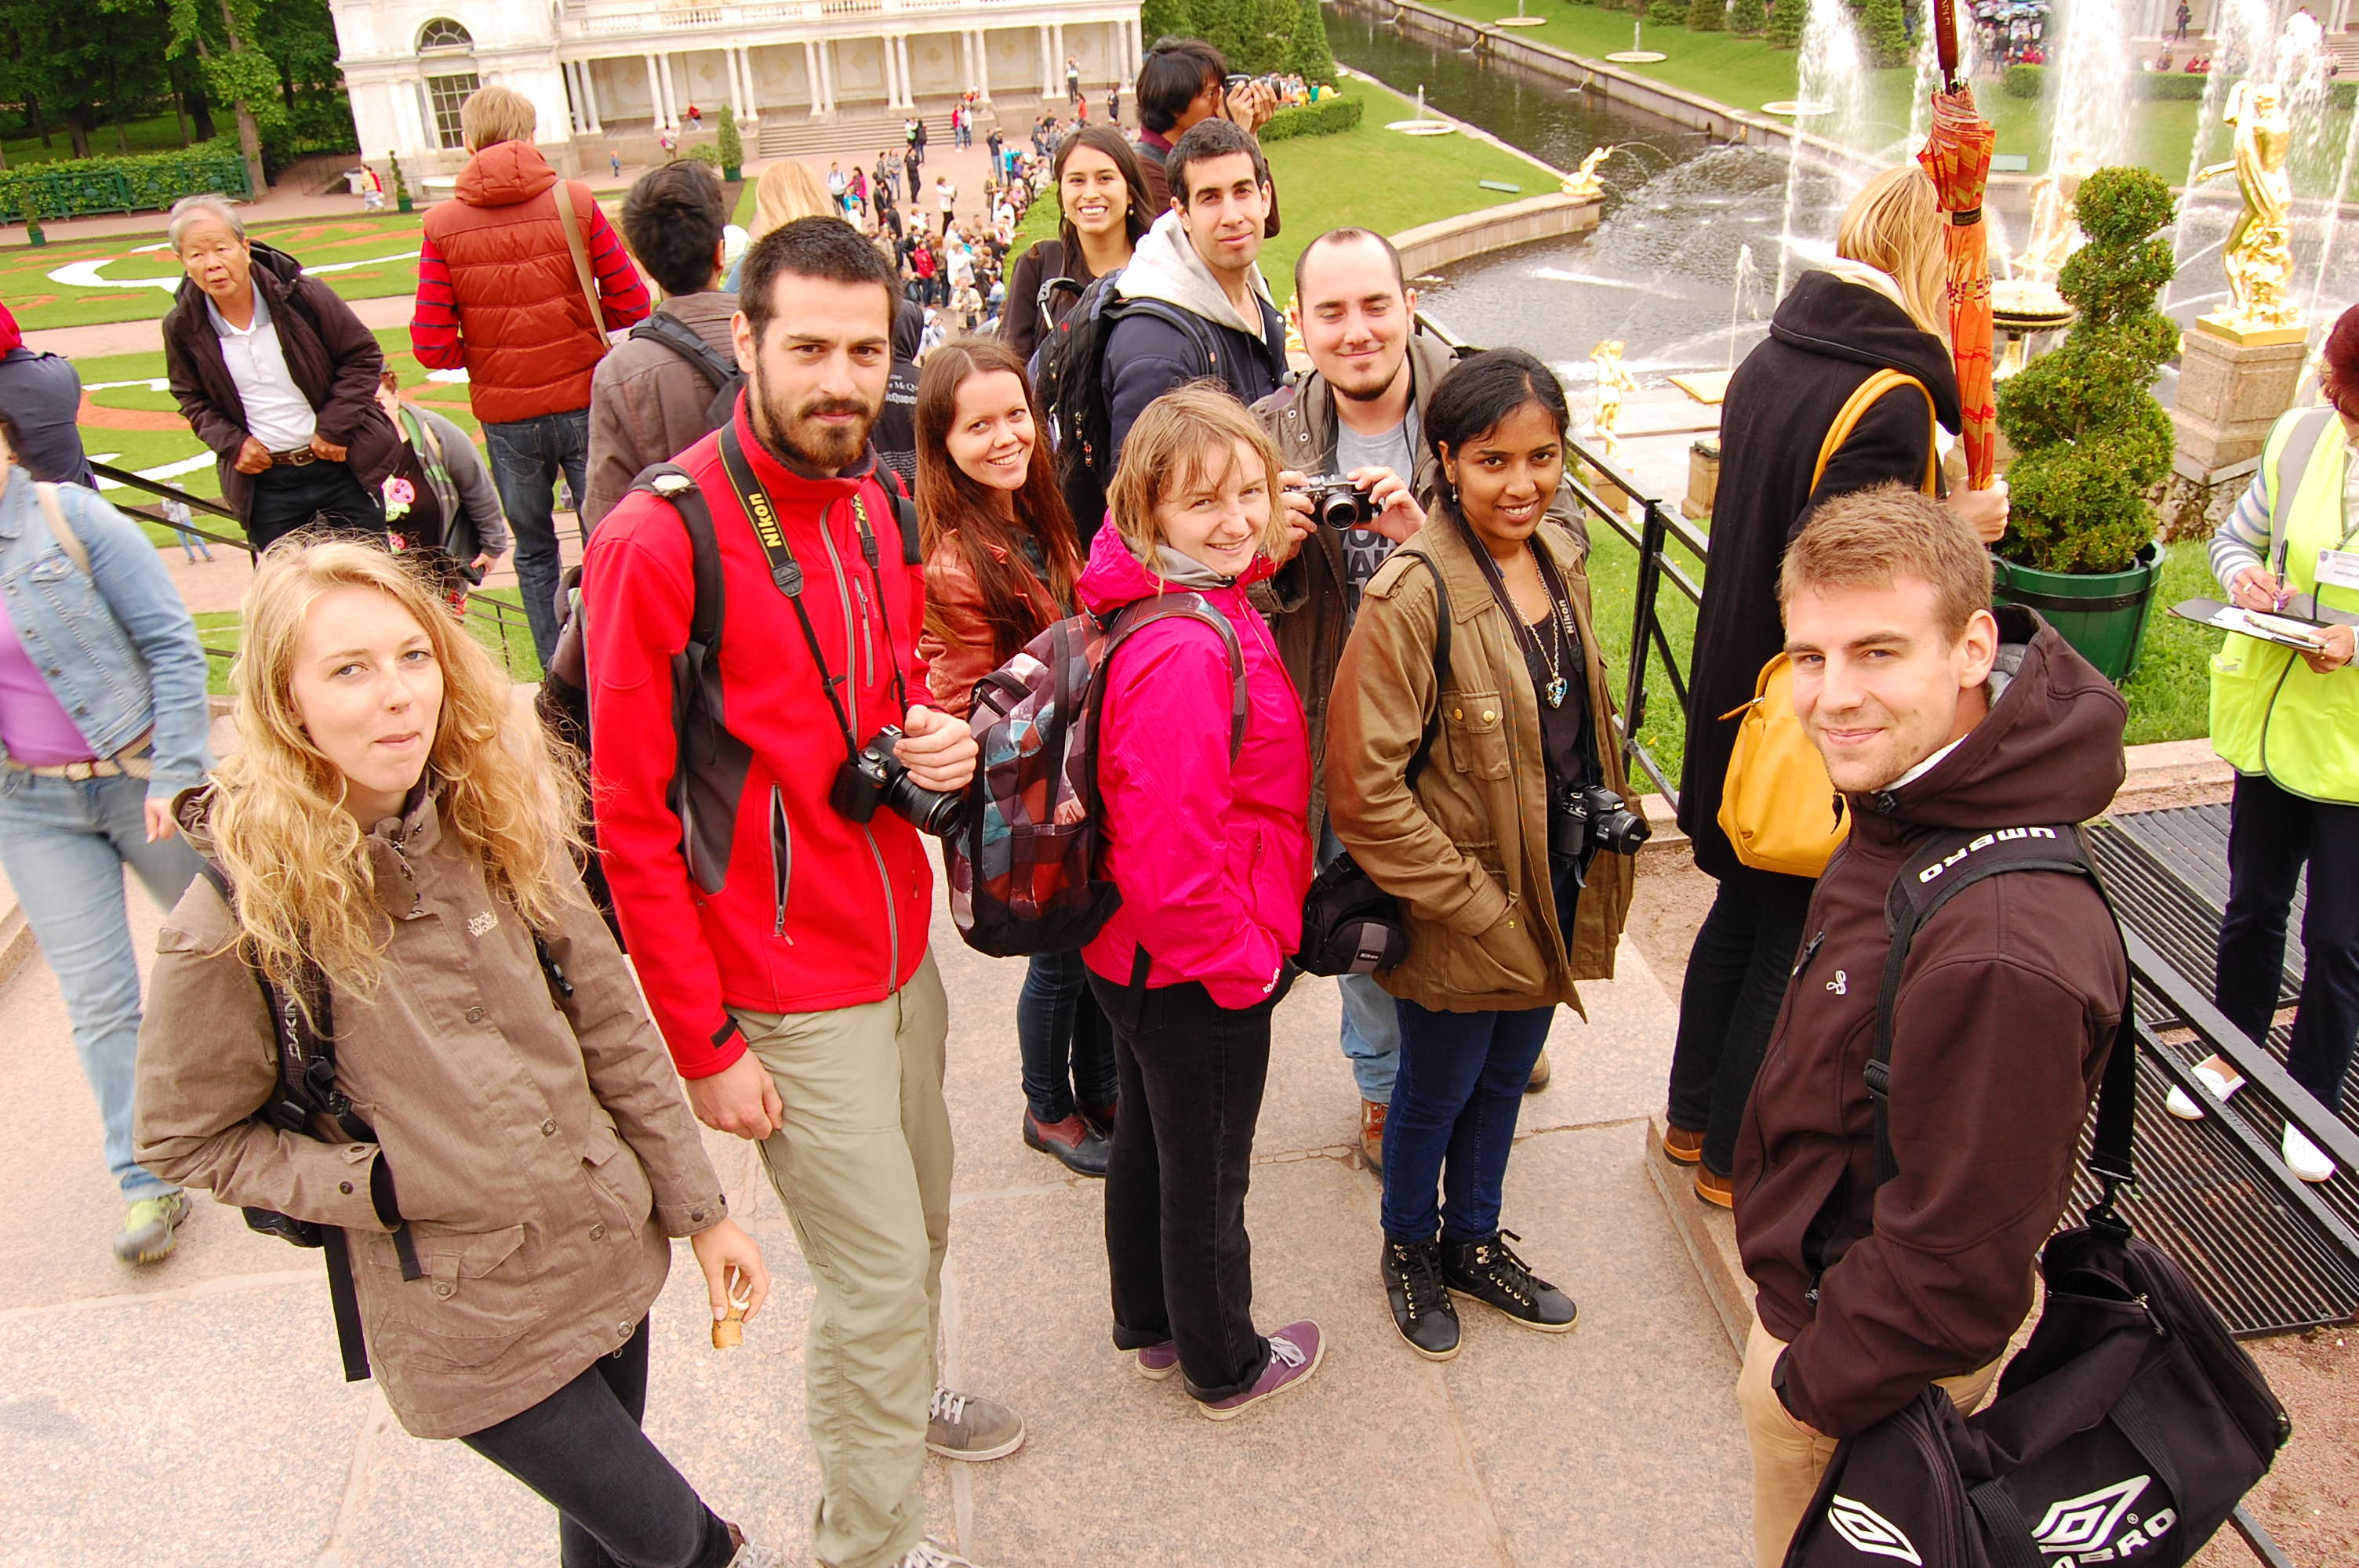
\includegraphics[width=0.45 \textwidth]{media/front_picture.jpg}
\\
\end{wrapfigure}
	
\NewsItem{Author's thoughts} % Main next item title
\vspace{3pt} % Some extra whitespace since there is no author as for the news in the body of the newsletter
\textit{
%12345678901234567890123456789012345678901234567890123456789012345678901234567890
Before going abroad, to pursue my Master's degree, I was living in tiny 
paradise called Cyprus. 
A little sandy island in the Mediteranian sea surrounded by three continents, 
offering strong sun light most of the year, amazing beaches, good-hearted people 
with great hospitality, chill and easy going life-style. 
However, the world was much bigger and attractive, in many and different sense, than 
I initially thought it would be.
This came like a flash light upon me when I visited four different countries 
in the context of my studies. 
I never thought before that: travelling; meeting new people; learning new things; 
accepting facts and mentalities from different cultures; will be an exciting and 
a large part of my dialy life. 
I have met people who gained my utmost trust and respect, and no matter how far 
away they are now they are still close and always in my thoughts.   
}
\par\hfill --- Stefanos Georgiou
\end{minipage}
\end{center}

\vspace{0.5cm}
\SepRule % Small horizontal rule after the main news item
\vspace{0.5cm}

%\setlength{\columnsep}{16pt} % Uncomment to manually change the white space between columns
\begin{multicols}{3} % Begin the three-column layout

%----------------------------------------------------------------------------------------
%	OTHER NEWS
%----------------------------------------------------------------------------------------

\NewsItem{What I was thinking?}
\NewsAuthor{Stefanos Georgiou}

%12345678901234567890123456789012345678901234567890123456789012345678901234567890
Growing in a small island (\textit{i.e.} Cyprus), I had a limited knowledge regarding 
the vast experience, new ideas, and cultural benefits I could assimilate while 
travelling abroad. 
Being in the last year of my under graduate studies, at the University of Cyprus, 
I had an aim of doing my post graduate degree in United Kingdom or any another 
English speaking country. 
In addition, alongside with the University, I had full time barista responsibilities 
at Starbucks cafeteria to collect money for my studies. 
While being in a family of six, with four sibiling, I believed it was important 
to get funds by any means to reduce the burden on my parents for doing my post graduate 
degree. 
The opportunity was given, to do my studies, while being eligible and qualified to 
receive a Erasmus Mundus scholarship, after I applied for {\sc perccom} (PERvasive 
Computing and COMmunications for sustainable development) program. 
A fact that made me super happy and left a huge smile on my face for many days.


%12345678901234567890123456789012345678901234567890123456789012345678901234567890
The above-mentioned Master program offered studies with the subject of GreenIT and 
sustainable development with the opportunite of studying in four different counties 
(France, Finland, Russia, and Sweden) for 18 student for the duration of two years. 
Moreover, it was a unique chance to meet people from different cultures and backgrounds 
since it was an international program and one of its purpose was of bringing together 
students from various countries. 
However, a bit skeptical about my choice, as a person who never livied abroad and 
who do not even know how to cook, I took the decision of exiting my confort zone 
and in the Semptember of 2013 I started my studies abroad. 
But who would know that I will end-up addicted in living abroad and having the 
travelling aspect as part of my life?


%12345678901234567890123456789012345678901234567890123456789012345678901234567890
During these two years of my post graduate studies, I acquired knowledge and 
experience that I would never had if I only stayed in a tiny island. 
My purpose is to share and motivate youngsters to get out of their comfort zone, 
travel a lot without thinking too much, meet a bunch of crazy people with no limits, 
and never forget to take your smile whenever you go or whatever the situation it is, 
becuase, in the end, \textit{we are just instances in this world and we 
should try to make all the best out of it}!


%-----------------------------------------------------------
\NewsItem{First stop: France}
% Talk about your meeting with Fisayo and how this friendship evolved during this time 
%12345678901234567890123456789012345678901234567890123456789012345678901234567890
France, the country of great wines, delicious cheese, funny english accent, 
and kind people was the first stop of my studies. 
More specifically, the city Nancy (located in the Northen France) offered its hospitality 
for the 18 {\sc perccom} students. 
The dream team composed from three Frenches, two Nigerians, two Indians, two Bangladeshi, two 
Indonitians, a German, a Peruvian, a Ukranian, a Romanian, a Vietnamese, and a 
Cypriot/Hungarian (myself).  


\begin{center}
	\includegraphics[width=0.32\textwidth]{media/strasbourg.jpg}
	\par\textit{City of Strasbourg}
\end{center} 

%12345678901234567890123456789012345678901234567890123456789012345678901234567890
I arrived in Nancy late in the evening, being exhausted from the trip, sweaty and 
dirty, and more importantly super hungry! 
That was my first encounter with Fisayo Caleb Oluwagboye, a guy from Nigeria also 
a student in my program about the same age as I. 
A kind, smart, and good-hearted person who is a very dear friend of mine 
and who later on he asked me to become his best man for his wedding.    
Even now (3 years after the Masters), we regularly speak over skype, or we try to 
meet at least once a year. 
Long story short, he was the first person who cooked for my while staying abroad 
once he realized how hungry I was. 
After that day we where always going out together, he was the person I trusted to 
speak my mind and the things that were bothering me like relationships, family staff, 
or studies. 


%12345678901234567890123456789012345678901234567890123456789012345678901234567890 
Our studies, in the University of Lorraine, where intense since we had to 
follow lectures eight hours almost every day. 
The French education system consistent mainly from long hours of lectures and less 
of homework. 
In addition, you had to speak formally with most of the professors compare to the 
Scandinavian Universities. 
We received most of the student guidance in the French Universities from our 
cohorts' students, Alexandre De Masi, Baptiste Louis, and Dorine Petit. 
Alexandre was our group's techno-freak, he was always connected and following 
every step of different technological advancements, but, mainly in the communications 
field. 
Baptiste was our group's \textit{princess}, a nick name that everybody liked and used. 
The nick name was given be me and Dorine while searching for a picture with the ``thank 
you'' description and the pricess word was also written there. 
Dorine was our group's dance addict, she was always willing to help us while 
staying in France, and she was reponsible for writing the {\sc perccom}'s blog and 
news.
These three were the people who mainly help us to bypass the hard French conversations 
in different domains gave us the first flavor of France while partying and organizing 
social events with them. 


\begin{center}
	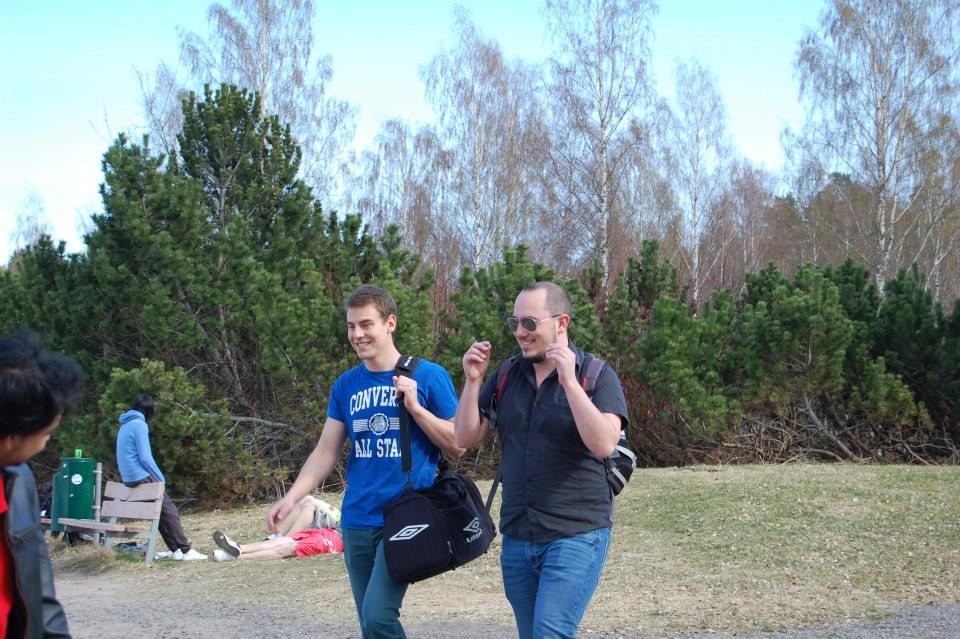
\includegraphics[width=0.32\textwidth]{media/baptiste_alex.jpg}
	\par\textit{Baptiste and Alexandre}
\end{center} 


%12345678901234567890123456789012345678901234567890123456789012345678901234567890
During our stay in France, we had also visited winery villages where the French 
speciallity lies. 
Those amazing places where you can get tipshy while testing the different varietions 
among the most excellent wines from the long term knowledge and inheritance that 
France offers to the world. 
The locals tried to help us to understand what are the differences of a good wine 
and how we should handle it based on its age. 
For instance, the oldest a red wine gets the more gentle gestures you have to use and 
less time is required to let it ``breathe''. 
We also learned that the difference of champagne against the other sparkling wines 
is nothing more than the production place, the region of Champagne. 
However, with our still immature and youngster nature we where only focus on getting 
drunk and having fun instead, I still feel lucky that I remember all the above 
information that I am currenly sharing. 


\begin{center}
	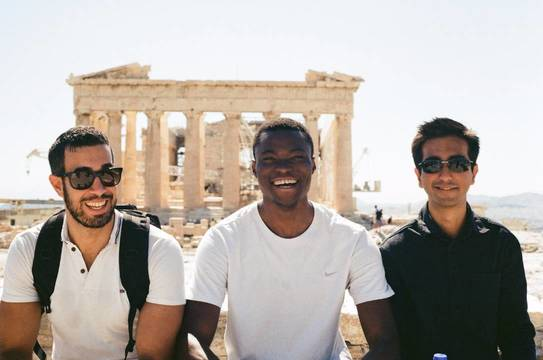
\includegraphics[width=0.32\textwidth]{media/stef_fisayo_rohan.jpg}
	\par\textit{I am left, Fisayo mid, and Rohan right}
\end{center}


%12345678901234567890123456789012345678901234567890123456789012345678901234567890
Another great experience that we had in France was the international evening 
we organized among the {\sc perccom} students at Alexandre's apartment. 
The aim was to bring traditional food and alchoolic drinks from our home countries 
and let everyone to have a taste from it. 
We tasted food from approximetely eleven various kitchens, the apartment of our 
host had smells from different spices and food for at least a week. 
I guess these smells also disturebed Alexandre's sleep since for some time he look 
really sleepy, or maybe it was the intense courses from our University with the 
combination of French professors accent while trying to teach in english.  
Nevertheless, we extended the night by having some beers at a local pub. 
As a non-beer drinker, I decided to try one, however, the options weres various 
and all unknown to me. 
That was the time when one of our fellows, Vlad (Romanian scout guy who was wearing a 
red characteristic jacket, drinking beers like water, and skillful programmer), 
told me the fantastic quote that I even use nowadays. 
\textit{``Stefanos, when don't know which one to pick just go for the blondes, 
	they are always the good choice''.} 
By thinking of that quote again, I am not aware if he only meant that for beers.


%12345678901234567890123456789012345678901234567890123456789012345678901234567890
After the awesome first semester in France, we packed our stuff and travelled 
to the ice-cold Lappeenranta of Finland to start our next semester.


%-----------------------------------------------------------
\NewsItem{Second stop: Finland}
% Talk about the sauna parties, and the walk over the Saima lake.
% The city of thousand lakes and the sauna parties
%12345678901234567890123456789012345678901234567890123456789012345678901234567890
The country of the thousand lakes and two millions of saunas is Finland. 
Where people are quite, peaceful, bearly speaking to strangers, not making eye 
contact, and they feel you are invating their personal space if you stand too 
close to them. 
However, when they start drinking alchool and partying they become open and cheerful. 
   
   
%12345678901234567890123456789012345678901234567890123456789012345678901234567890 
In the beggining of January 2014, Finland welcomed our cohort with shony days 
and long nights. 
In the north, most of countries have long nights during winter times and long 
days during the summer times. 
Some common patterns of the Scandinavia countries are: sun is rare and a valuable; 
prices of alchoolic drinks and smokes are high due to taxation; eating in a 
restaurant is pricy; expensive bus tickets; getting a decend hair cut costs; 
high and education system; amazing public health service; busses on time; 
and every single person knew english and with a proper accent.
     

%12345678901234567890123456789012345678901234567890123456789012345678901234567890 
To reduce some of these aforementioned costs since we had a small scholarship and 
definetily not one that is enough for Scandinavian countries, we took some 
measurements. 
For example, we bought a complete hair cut kit and we entrusted out hair to 
Alexandre---how only had experience in cutting sheeps' fur as one time he said 
while being drunk.  
Worth to say for free hair cut it wasn't that...bad! 
To reduce the transportation fees, since I was leaving five kilometers away from 
the University, I used to walk everyday. 
Luckily the lake Saimaa, that one I had to pass by to get at the University, got 
frozen. 
Therefore, it offered a direct part to the University if someone was crazy enough 
to risk working on the frozen lake. 
However, a bit unconfortable initially, I took the big step and started everyday 
going to the University through the frozen Saimaa lake.

\begin{center}
	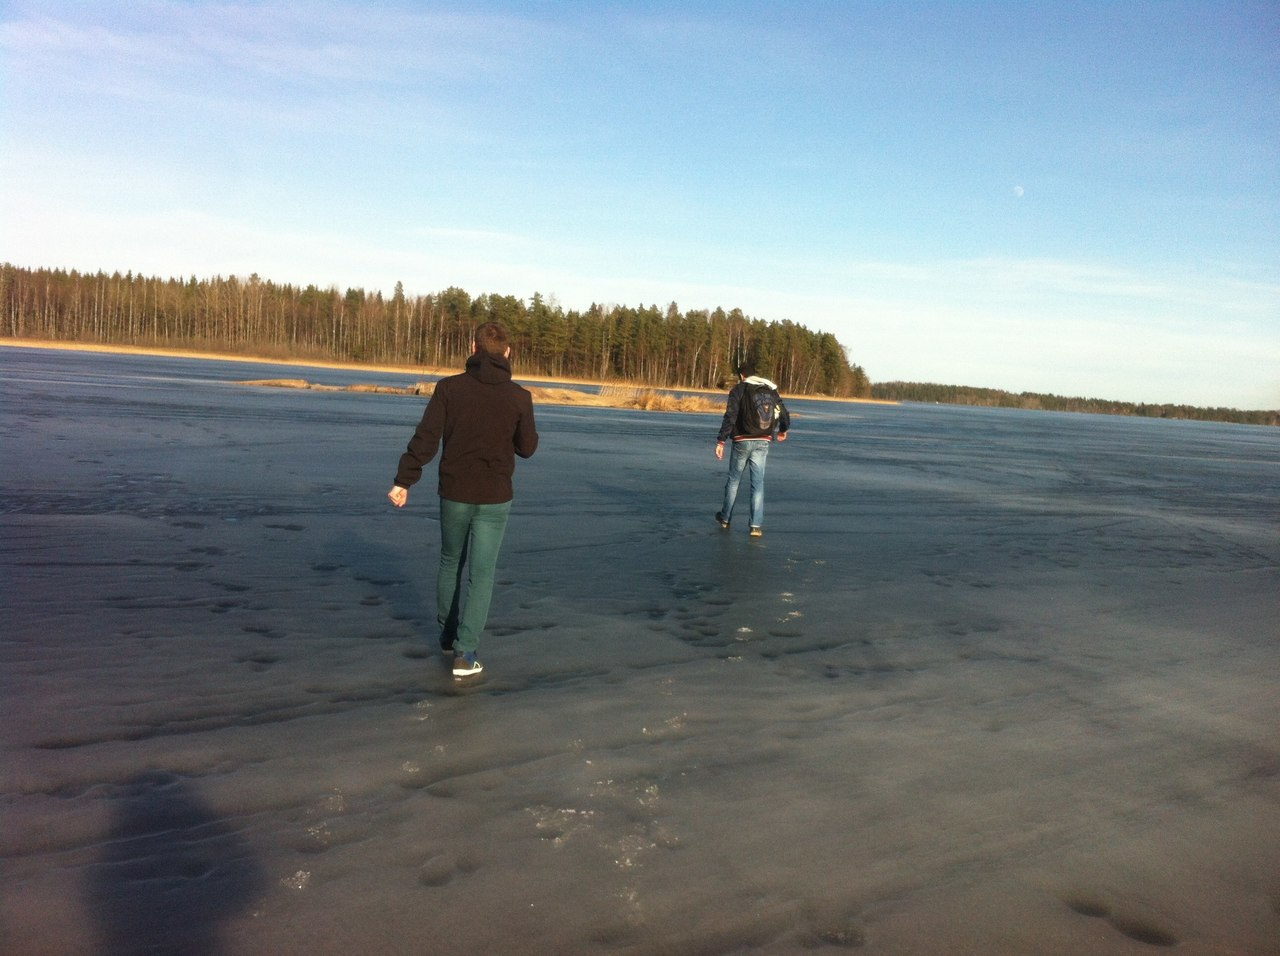
\includegraphics[width=0.32\textwidth]{media/walking_on_ice.jpg}
	\par\textit{Walking on a frozen lake to go home}
\end{center}


%-----------------------------------------------------------
\NewsItem{Third stop: Sweden}
% Talk about the figa, the hokey
% Where the coffee is a mandatory fact even after fast-food
% Boot camp 48 hours non-sleep

%-----------------------------------------------------------
\NewsItem{Forth stop: Russia}



%-----------------------------------------------------------
\NewsItem{What I have learned?}

%12345678901234567890123456789012345678901234567890123456789012345678901234567890
Once a professor of mine told \textit{``You can realize the 
	quality of a culture when coming across with something different 
	from its understanding''}. 
You show your quality based on how to accept something different and 
out of your understanding.
These words made more sense to me while studying with people that where different 
from me. 
We became close friends because we accepted each other and respected what was 
different from us. 
 




\begin{quotation} % Example of a quotation
\noindent{\Huge``}

\noindent\normalsize\textit{All those magical moments I spend during my 
	Masters in all these different countries are carved in deeply in my 
	memories and thoughts. 
	I wish I could term back time and re-live this enjoyable and unique 
	jounral over and over again.
}

\hfill{\Huge''}

\end{quotation}


\end{multicols}


\begin{center}
	\vspace{10pt}
	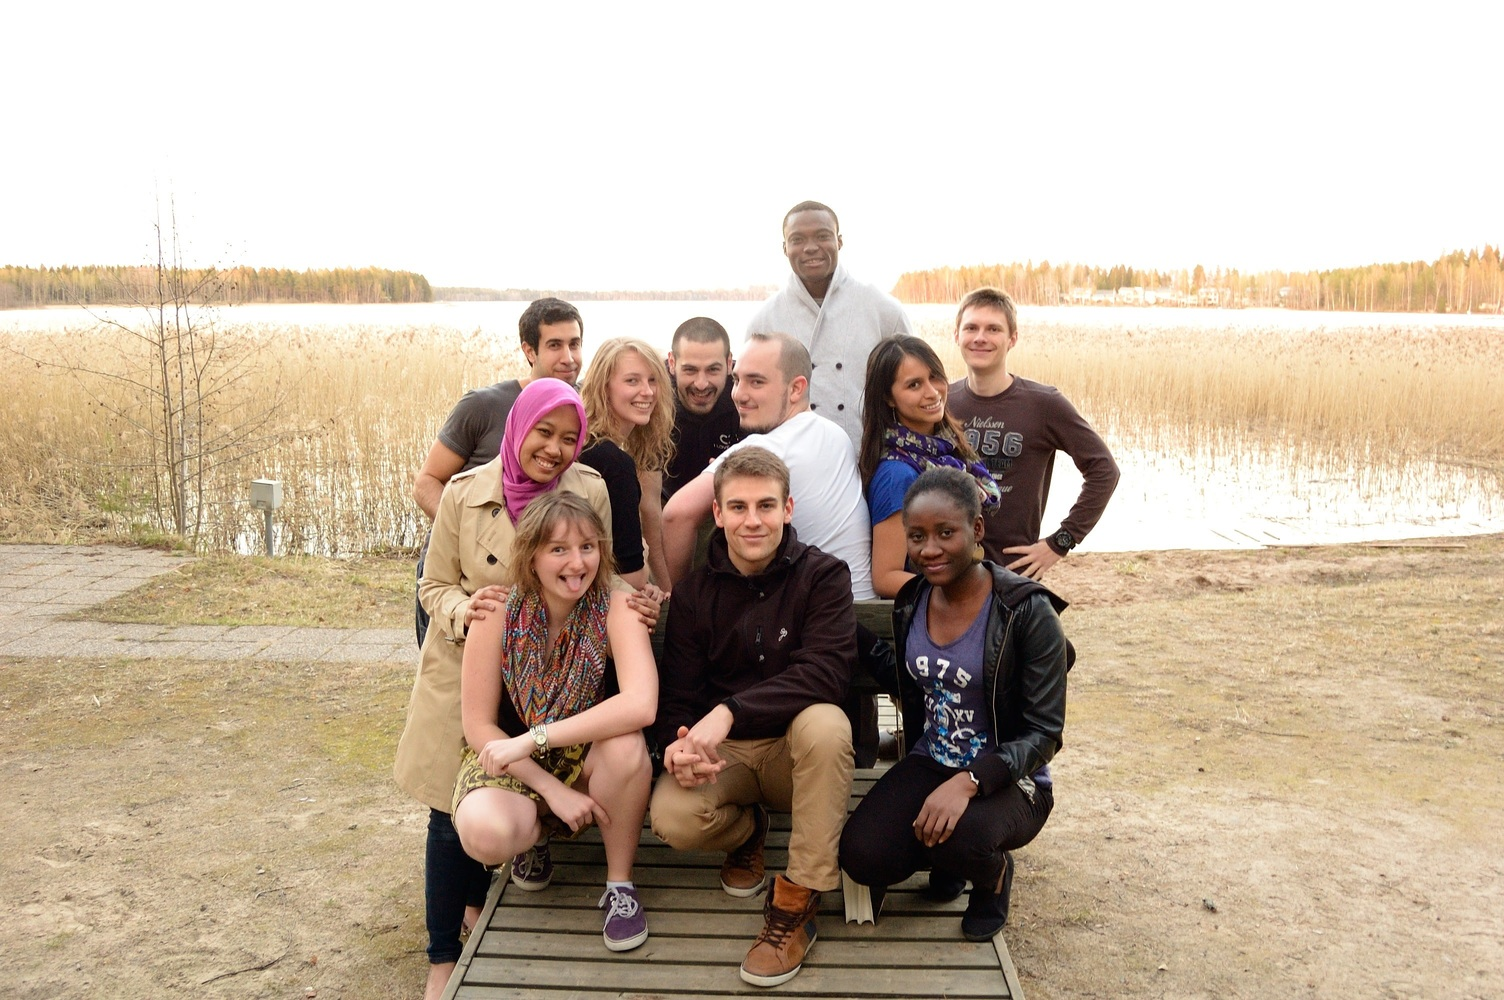
\includegraphics[width=0.8\linewidth]{media/perccom_family.jpg} % Example of an image taking up the total width of the page

	\vspace{10pt}
\end{center}
%----------------------------------------------------------------------------------------

\end{document} 